% Created 2022-09-20 mar 17:15
% Intended LaTeX compiler: pdflatex
\documentclass[11pt]{article}
\usepackage[utf8]{inputenc}
\usepackage[T1]{fontenc}
\usepackage{graphicx}
\usepackage{longtable}
\usepackage{wrapfig}
\usepackage{rotating}
\usepackage[normalem]{ulem}
\usepackage{amsmath}
\usepackage{amssymb}
\usepackage{capt-of}
\usepackage{hyperref}
\author{Semanticas}
\date{\textit{<2018-08-14 mar>}}
\title{C. A. L. P.}
\hypersetup{
 pdfauthor={Semanticas},
 pdftitle={C. A. L. P.},
 pdfkeywords={},
 pdfsubject={},
 pdfcreator={Emacs 27.1 (Org mode 9.5.2)}, 
 pdflang={English}}
\begin{document}

\maketitle



\section*{Introducción}
\label{sec:orgeab22ee}

\subsection*{Introducción}
\label{sec:orgd827289}
\begin{itemize}
\item \textbf{Sintaxis}: La forma y estructura de las expresiones, sentencias y
unidades del programa.
\item \textbf{Semántica}: El significado de las expresiones, sentencias, y
unidades del programa.
\item Sintaxis y Semántica proveen una Definición del Lenguaje
\begin{itemize}
\item Usuarios de una Definición del Lenguaje
\begin{itemize}
\item Otros diseñadores del Lenguaje
\item Implementadores
\item Programadores
\end{itemize}
\end{itemize}
\end{itemize}

\subsection*{Definición Formal de Lenguajes}
\label{sec:orge40f493}
\begin{itemize}
\item \textbf{Reconocedores}
\begin{itemize}
\item Un dispositivo de reconocimiento que lee cadenas del lenguaje y
decide si las cadenas de entrada pertenecen al Lenguaje.
\item Ejemplo, el analizador sintáctico de un compilador.
\end{itemize}
\item \textbf{Generadores}
\begin{itemize}
\item Un dispositivo que genera sentencias de un lenguaje
\item Se puede determinar si la sintaxis de una sentencia particular es
correcta comparándola con la estructura del generador.
\end{itemize}
\end{itemize}
\subsection*{Métodos Formales de Describir la Sintaxis}
\label{sec:org1f3ca6d}
\begin{itemize}
\item Forma Backus-Naur y gramáticas libres de contexto
\begin{itemize}
\item El método mas conocido para describir la sintaxis de un Lenguaje
de Programación.
\end{itemize}
\item BNF Extendida
\begin{itemize}
\item Mejora la legibilidad de BNF
\end{itemize}
\item Gramáticas y Reconocedores
\end{itemize}

\subsection*{BNF y Gramáticas Libres de Contexto}
\label{sec:org930b9ea}
\begin{itemize}
\item Gramáticas libres de Contexto
\begin{itemize}
\item Desarrollado por Noam Chomsky a mediados de 1950s
\item Generadores de Lenguajes, medio de  describir la la sintaxis de
lenguajes naturales
\item Define clases de lenguajes
\end{itemize}
\item Forma Backus-Naur (1959)
\begin{itemize}
\item Inventado por John Backus para describir Algol 58
\item Árboles sintacticos - ambiguedad del lenguaje
\end{itemize}
\end{itemize}

\section*{Semántica Estática}
\label{sec:org2bcef72}

\subsection*{Gramáticas con atributos}
\label{sec:orgab65659}
\begin{itemize}
\item Las Gramáticas Libres de Contexto (GLC) no pueden describir toda la sintaxis de
los lenguajes de programación.
\item Agregados a GLC para introducir información semántica en los árboles sintácticos
\item Principal aporte de las Gramáticas con atributos
\begin{itemize}
\item Especificación de la semántica estática
\item Diseño de Compiladores (chequeo de semántica estática)
\end{itemize}
\end{itemize}

\subsection*{Gramáticas con atributos: Definición}
\label{sec:orgd4fb997}
\begin{itemize}
\item Una Gramática con atributos es una gramática libre de contexto \(G =
  (S,N,T,P)\) con los siguientes agregados:
\begin{itemize}
\item Por cada símbolo de gramática \(x\) hay un conjunto \(A(x)\) de
valores de atributos
\item Cada regla tiene un conjunto de funciones que definen ciertos
atributos de los no terminales en la regla
\item Cada regla tiene un conjunto posiblemente vacío de predicados para
chequear la consistencia de los atributos
\end{itemize}
\end{itemize}

\subsection*{Gramáticas con atributos: Definición}
\label{sec:org436f531}
\begin{itemize}
\item Sea \(X_0 \to X_1 ... X_n\) una regla de la gramática libre de contexto
\item Funciones de la forma \(S(X_0) = f(A(X_1), ... , A(X_n))\) definen
\emph{atributos sintetizados}
\item Funciones de la forma \(I(X_j) = f(A(X_0)), ... , f(A(X_{j-1}))\) para \(i
  <= j <= n\), definen \emph{atributos heredados}
\item Inicialmente hay \emph{atributos intrínsecos} en las hojas de los árboles sintácticos
\end{itemize}

\subsection*{Gramáticas con atributos: Un Ejemplo}
\label{sec:org4316ad3}
\begin{itemize}
\item Sintaxis
\begin{itemize}
\item <assign> \(\to\) <var> = <expr>
\item <expr> \(\to\) <var> + <var> | <var>
\item <var> \(\to\) A | B | C
\end{itemize}

\item tipo-real: sintetizado por <var> y <expr>
\item tipo-esperado: heredado por <expr>
\end{itemize}

\begin{center}
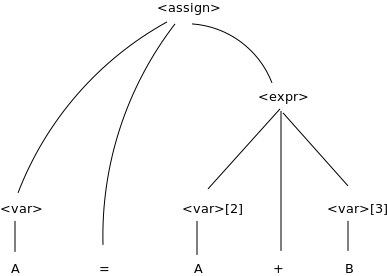
\includegraphics[width=.9\linewidth]{attribgram1.png}
\end{center}

\subsection*{Gramáticas con atributos: Un Ejemplo}
\label{sec:orgc838a29}
\begin{enumerate}
\item Regla sintáctica: <assign> \(\to\) <var> = <expr>
\begin{itemize}
\item Regla semántica: <expr>.tipo-esperado \(\leftarrow\) <var>.tipo-real
\end{itemize}
\item Regla sintáctica: <expr> \(\to\) <var>[ 2] + <var>[ 3]
\begin{itemize}
\item Regla semántica: <expr>.tipo-real  \(\leftarrow\)

if (<var>[ 2].tipo-real = int) and (<var>[ 3].tipo-real = int)
then int else real end if

\item Predicado: <expr>.tipo-real = <expr>.tipo-esperado
\end{itemize}

\item Regla sintáctica: <expr> \(\to\) <var>
\begin{itemize}
\item Regla semántica: <expr>.tipo-real \(\leftarrow\) <var>.tipo-real
\item Predicado: <expr>.tipo-real = <expr>.tipo-esperado
\end{itemize}

\item Regla sintáctica: <var> \(\to\) A | B | C
\begin{itemize}
\item Regla semántica:  <var>.tipo-real \(\leftarrow\) lookup (<var>.string)
\end{itemize}
\end{enumerate}

\subsection*{Gramáticas con atributos}
\label{sec:org9f2ae14}
\begin{itemize}
\item ¿Cómo se computan los valores de atributos?
\begin{itemize}
\item Si todos los atributos fueran heredados, el árbol podría ser
completado en un orden \emph{top-down}.
\item Si todos los atributos fueran sintetizados, el árbol podría ser
completado en un orden \emph{bottom-up}
\item En muchos casos, ambos casos de atributos son utilizados y se
necesita una combinación de ambos órdenes.
\end{itemize}
\end{itemize}

\begin{center}
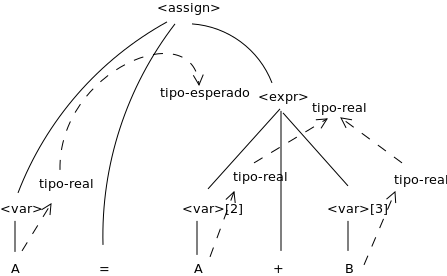
\includegraphics[width=.9\linewidth]{attribgram2.png}
\end{center}

\subsection*{Gramáticas con atributos}
\label{sec:org0ee1416}
\begin{enumerate}
\item <var>.tipo-real \(\leftarrow\) look-up(A) (Regla 4)
\item <expr>.tipo-esperado \(\leftarrow\) <var>.tipo-real (Regla 1)
\item \begin{itemize}
\item <var>[ 2].tipo-real \(\leftarrow\) look-up(A) (Regla 4)
\item <var>[ 3].tipo-real \(\leftarrow\) look-up(B) (Regla 4)
\end{itemize}
\item <expr>.tipo-real \(\leftarrow\) int o real (Regla 2)

\item <expr>.tipo-esperado = <expr>.tipo-real es VERDADERO o FALSO (Regla 2)
\end{enumerate}

\begin{center}
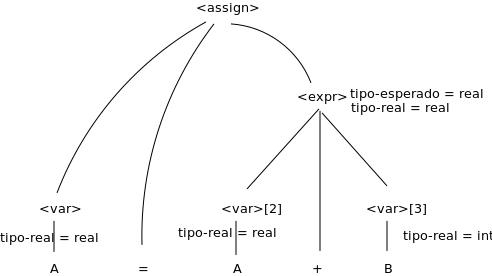
\includegraphics[width=.9\linewidth]{attribgram3.png}
\end{center}

\section*{Semántica Dinámica}
\label{sec:org0df1f6c}

\subsection*{Métodos Desarrollados}
\label{sec:orgcb2c3eb}
\begin{itemize}
\item Semántica Operacional
\begin{itemize}
\item Operaciones en una máquina abstracta
\end{itemize}
\item Semántica Denotacional
\begin{itemize}
\item Usa funciones para especificar la semántica, los programas se
convierten en funciones para poder aplicar la teoría de funciones recursivas
\end{itemize}
\item Semántica Axiomática
\begin{itemize}
\item Aplica la lógica formal: afirmaciones (aserciones) para describir
suposiciones y resultados deseados
\item Los axiomas o reglas de inferencia son usados en cada tipo de
sentencias.
\end{itemize}
\end{itemize}


\subsection*{Semántica Operacional}
\label{sec:org963848d}
\subsubsection*{Semántica Operacional}
\label{sec:org8bb72d4}
\begin{itemize}
\item Describe el significado de un programa ejecutando sus sentencias
sobre una máquina, simulada o real. Los cambios en el estado de la
máquina (registros, memoria, etc) define el significado de la sentencia.
\item Para el uso de una semántica operacional en un lenguaje de alto
nivel se necesita una máquina virtual
\begin{itemize}
\item Un intérprete de hardware puro podría ser muy costoso.
\item Un intérprete de software puro también tiene problemas
(dependiente de la máquina )
\end{itemize}
\item Una mejor alternativa: Una simulación completa de la computadora
\begin{itemize}
\item Construir un traductor del codigo fuente a un codigo maquina de
una computadora idealizada
\item Construir un simulador para la computadora idealizada
\end{itemize}
\end{itemize}

\subsubsection*{Semántica Operacional}
\label{sec:org534c97b}

\begin{itemize}
\item Simulador de Prolog en Prolog
\end{itemize}

\begin{verbatim}
mi(true).
mi((A,B)) :-
	mi(A),
	mi(B).
mi(Goal) :-
	Goal \= true,
	Goal \= (_,_),
	clause(Goal, Body),
	mi(Body).
\end{verbatim}

\begin{itemize}
\item Evaluación:
\begin{itemize}
\item Bueno usado informalmente.
\item Extremadamente complejo usado formalmente.
\end{itemize}
\end{itemize}

\subsection*{Semántica Denotacional}
\label{sec:orgcaf47ef}
\subsubsection*{Semántica Denotacional}
\label{sec:org3a1e310}
\begin{itemize}
\item Basado en la teoría de funciones recursivas
\item El método de descripción semántica mas abstracto
\item Originalmente desarrollado por Scott y Strachey (1970)
\item El proceso de construir una especificación denotacional para un
lenguaje es definir un objeto matemático por cada entidad del Lenguaje
\begin{itemize}
\item Define una función que relaciona instancias de las entidades del
lenguaje con instancias de los objetos matemáticos correspondientes
\end{itemize}
\item El significado de las construcciones del lenguaje son definidos solo
por los valores de las variables del programa
\end{itemize}

\subsubsection*{Semántica Denotacional vs Semántica Operacional}
\label{sec:org4cef103}
\begin{itemize}
\item En la semántica operacional los cambios de estado son definidos por
algoritmos codificados
\item En la semántica denotacional los cambios de estado son definidos por
funciones matemáticas rigurosas.
\item El estado de un programa son los valores de todas las variables
actuales  \(s = { < i_1,v_1 >,< i_2,v_2 >, ... ,< i_n,v_n > }\)
\item Sea  \emph{VARMAP} una función que, cuando recibe un nombre de variable y
un estado retorna el valor actual de esa variable \({VARMAP}(i_j, s) = v_j\)
\end{itemize}

\subsubsection*{Números Decimales}
\label{sec:orgf40bff1}
\begin{itemize}
\item <dec-num> \(\to\) 0 | 1 | 2 | 3 | 4 | 5 | 6 | 7 | 8 | 9 |
\item M\textsubscript{dec} ('0') = 0,  M\textsubscript{dec} ('1') = 1, \ldots{} , M\textsubscript{dec} ('9') = 9
\item M\textsubscript{dec} ( <dec-num> '0') = 10 * M\textsubscript{dec} ( <dec-num> )
\item M\textsubscript{dec} ( <dec-num> '1') = 10 * M\textsubscript{dec} ( <dec-num> ) + 1
\item \ldots{}
\item M\textsubscript{dec} ( <dec-num> '9') = 10 * M\textsubscript{dec} ( <dec-num> ) + 9
\end{itemize}

\subsubsection*{Expresiones}
\label{sec:org9085d78}
\begin{itemize}
\item relaciona expresiones a Z \(\cup\) \{ error \}
\item suponiendo que las expresiones son números decimales, variables, o
expresiones binarias teniendo un operador aritmético y dos
operandos, cada uno de los cuales puede ser una expresión.
\item M\textsubscript{e} ( < expr >, s) = case < expr > of 
\begin{itemize}
\item < dec-num > \(\to\) M\textsubscript{dec} ( < dec-num > , s)
\item < var > \(\to\) if VARMAP(< var >, s)
\item < binary-expr > \(\to\) 
\begin{itemize}
\item if (M\textsubscript{e}(< binary-expr > . <left-expr > , s) = undef
\begin{itemize}
\item OR M\textsubscript{e}(< binary-expr > . < right-expr > , s) = undef)
\end{itemize}
\item then error
\item else
\begin{itemize}
\item if (< binary-expr >.< operator > = ‘+’ then
\item M\textsubscript{e}(< binary-expr >.< left-expr >, s) + M\textsubscript{e}(< binary-expr >.<
right-expr >, s)
\item else M\textsubscript{e}(< binary-expr >.< left-expr >, s) * M\textsubscript{e}(< binary-expr
>.< right-expr >, s)
\end{itemize}
\end{itemize}
\end{itemize}
\item \ldots{}
\end{itemize}

\subsubsection*{asignación}
\label{sec:org2590849}
\begin{itemize}
\item M\textsubscript{a} ( X := E, s) = 
\begin{itemize}
\item if M\textsubscript{e}(E, s) = error
\begin{itemize}
\item then error
\item else s' = \{ < i\textsubscript{1}',v\textsubscript{1}' >, < i\textsubscript{2}',v\textsubscript{2}' >, \ldots{} , < i\textsubscript{n}',v\textsubscript{n}' >\},
\begin{itemize}
\item where for j = 1, 2, \ldots{} n,
\begin{itemize}
\item v\textsubscript{j}' = varmap(i\textsubscript{j}, s) if i\textsubscript{j} <> x
\begin{itemize}
\item = M\textsubscript{e}(E, s) if i\textsubscript{j} = x
\end{itemize}
\end{itemize}
\end{itemize}
\end{itemize}
\end{itemize}
\end{itemize}

\subsubsection*{Ciclo 'while'}
\label{sec:org7ae08fb}
\begin{itemize}
\item M\textsubscript{l}(while B do L, s) =
\begin{itemize}
\item if M\textsubscript{b}(B, s) = undef
\begin{itemize}
\item then error
\item else if M\textsubscript{b}(B, s) = false
\begin{itemize}
\item then s
\item else if M\textsubscript{sl}(L, s) = error
\begin{itemize}
\item then error
\item else M\textsubscript{l}(while B do L, M\textsubscript{sl}(L, s))
\end{itemize}
\end{itemize}
\end{itemize}
\end{itemize}
\end{itemize}

\subsubsection*{Ciclo}
\label{sec:org2b5240e}
\begin{itemize}
\item El significado del ciclo es el valor de las variables del programa
después de que las sentencias del ciclo han sido ejecutadas el
número prescrito de veces, asumiendo que no ha habido errores
\item En esencia el ciclo ha sido convertido de iterativo a recursivo,
donde el control recursivo es definido por otra función recursiva de estados
\item La recursión comparada con la iteración es mas facil de describir
con rigor matemático
\end{itemize}

\subsubsection*{Evaluación}
\label{sec:org75c80e9}
\begin{itemize}
\item Puede ser usado para probar la corrección de programas
\item Provee un modo riguroso de pensar los programas
\item Puede ser una ayuda al diseño de lenguajes
\item Ha sido usado en sistemas de generación de compiladores
\item A causa de su complejidad es de poco uso para los usuarios del lenguaje
\end{itemize}



\subsection*{Semántica Axiomática}
\label{sec:org75e1b8c}

\subsubsection*{Semántica Axiomática}
\label{sec:org2680c9e}
\begin{itemize}
\item Basado en Lógica Formal (cálculo de predicados)
\item Propósito original: Verificación formal de programas
\item Axiomas o reglas de inferencia son definidas para cada tipo de
sentencia del lenguaje (para permitir transformaciones de
expresiones a otras expresiones)
\item Las expresiones son llamadas \emph{aserciones} (afirmaciones)
\end{itemize}

\subsubsection*{Semántica Axiomática}
\label{sec:org0204334}
\begin{itemize}
\item Una aserción antes de una sentencia (una \emph{precondición} establece
las relaciones y restricciones entre variables que son verdaderas en
ese punto de la ejecución
\item Una aserción que sigue a una sentencia es una \emph{postcondición}
\item Una \emph{precondición mas débil} es la menos restrictiva precondición
que garantiza la postcondición
\end{itemize}

\subsubsection*{Semántica Axiomática}
\label{sec:orgbd21fc1}
\begin{itemize}
\item La Forma es \{P\} sentencia \{Q\}
\item Un ejemplo
\begin{itemize}
\item a = b + 1 \{a > 1\}
\item una posible precondición: \{b > 10)
\item \emph{precondición mas débil}: \{b > 0\}
\end{itemize}
\end{itemize}

\subsubsection*{Proceso de prueba de programa}
\label{sec:orgacbbe55}
\begin{itemize}
\item La postcondición para el programa entero es el resultado deseado
\begin{itemize}
\item Se trabaja hacia atrás a través del programa hasta la primer
sentencia. Si la precondición sobre la primer sentencias está
inferida por la especificación de entrada del programa, entonces
el programa es correcto.
\end{itemize}
\end{itemize}

\subsubsection*{Axiomas}
\label{sec:org54048c9}
\begin{itemize}
\item Un axioma para la asignación
\begin{itemize}
\item ( x = E ): \(\{Q_{x \to E}\} \ x = E \ \{Q\}\)
\end{itemize}
\item La regla de la Consecuencia

\[ \frac{ \{P\} \ S \ \{Q\}, P' \Rightarrow P, Q \Rightarrow
  Q'}{\{P'\} \ S \ \{Q'\}} \]
\end{itemize}

\subsubsection*{Axiomas}
\label{sec:org47926a1}
\begin{itemize}
\item \(x = 2 * y - 3 \{x > 25 \}\)
\item \(2 * y - 3 > 25\)
\item \(y > 14\)
\item \(x = x + y - 3 \{x > 10 \}\)
\item \(x + y - 3 > 10\)
\item \(y > 13 - x\)
\end{itemize}

\subsubsection*{Axiomas}
\label{sec:org6e5345f}
\[ \frac{ \{x > 3\} \ x = x - 3 \ \{x > 0\}, (x > 5) \Rightarrow (x >
  3), (x > 0) \Rightarrow (x > 0)}{\{x > 5\} \ x = x - 3 \ \{x > 0\}} \]

\subsubsection*{Axiomas}
\label{sec:org4527a15}
\begin{itemize}
\item Una regla de inferencia para secuencias
\begin{itemize}
\item \(\{P1\} S1 \{P2\}\)
\item \(\{P2\} S2 \{P3\}\)
\end{itemize}
\end{itemize}

\[ \frac{ \{P1\} \ S1 \ \{P2\}, \{P2\} \ S2 \ \{P3\}}{\{P1\} \ S1;S2 \ \{P3\}} \]

\subsubsection*{Axiomas}
\label{sec:orgccae7ab}
\begin{itemize}
\item \(y = 3 * x + 1\);

\item \(x =  y + 3\);

\item \(\{ x < 10 \}\)
\end{itemize}

La precondición para la segunda asignación es \(y < 7\) la cual es
usada como postcondición para la primer sentencia. La precondición
para la primera asignación puede ser computada 

\begin{itemize}
\item \(3 * x + 1 < 7\)

\item \(x < 2\)
\end{itemize}

\subsubsection*{Axiomas}
\label{sec:orge0e3476}
\begin{itemize}
\item regla de inferencia para sentencias de selección  \emph{if}

\{P\} \textbf{if} B \textbf{then} S1 \textbf{else} S2 \{Q\}
\end{itemize}

\[ \frac{ \{B \ and \ P \} \ S1 \ \{Q\}, \{(not B) \ and \ P\} \ S2 \ 
\{Q\}}{\{P\} \ if \ B \ then \ S1 \ else \ S2 \ \{Q\}}\]

\subsubsection*{Ejemplo}
\label{sec:orgde11d1e}
\begin{itemize}
\item \textbf{if} \(x > 0\) \textbf{then} \(y = y - 1\) \textbf{else} \(y =  y + 1\)
\end{itemize}
\begin{itemize}
\item con la postcondición \(\{ y > 0 \}\)
\item el axioma de asignación para la clausula \textbf{then}: \(y = y - 1  \{ y
  > 0 \}\)  produce \(\{ y - 1 > 0 \}\) o \(\{ y > 1 \}\)
\item el axioma de asignación para la clausula \textbf{else}: \(y = y + 1  \{ y
  > 0 \}\)  produce \(\{ y + 1 > 0 \}\) o \(\{ y > -1 \}\)
\item Como \(\{ y > 1 \} \Rightarrow \{ y > -1 \}\) la regla de
consecuencia nos permite usar \(\{ y > 1 \}\) como precondición
del total de la sentencia
\end{itemize}

\subsubsection*{Axiomas}
\label{sec:org675e4ce}
\begin{itemize}
\item Una regla de inferencia para un ciclo \emph{while}

\{P\} \textbf{while} B \textbf{do} S \textbf{end} \{Q\}
\end{itemize}

\[ \frac{ (I \ and \ B ) S \{I\} }{\{I\} \ while \ B \ do \ S \{I \
and (not B)\}} \]

donde \emph{I} es el \emph{invariante} (la hipótesis inductiva)

\subsubsection*{Axiomas}
\label{sec:org245dbd6}
\begin{itemize}
\item Características del \emph{invariante}: \emph{I} debe satisfacer las siguientes
condiciones:
\begin{itemize}
\item \(P \Rightarrow I\) el invariante debe ser inicialmente verdadero
\item \(\{I\} \ B \ \{I\}\) la evaluación de la parte booleana no
debe cambiar la validez de \emph{I}
\item \(\{I \ and \ B \} \ S \ \{I\}\) \emph{I} no cambia por la ejecución
del cuerpo del ciclo  iterativo
\item \((I \ and \ (not \ B)) \Rightarrow Q\) si \emph{I} es verdadero y
\emph{B} es falso es implicado \emph{Q}
\item El ciclo termina
\end{itemize}
\end{itemize}

\subsubsection*{Ejemplo}
\label{sec:org1ce24d2}
\begin{itemize}
\item \textbf{while} \(y <> x\) \textbf{do} \(y = y + 1\) \textbf{end} \(\{ y = x \}\)
\end{itemize}
\begin{itemize}
\item Para cero iteraciones la precondición mas débil es \(\{ y = x \}\)
\item Para una iteración es: \[ wp( y = y + 1, \{y = x\}) = \{ y + 1 = x \} = \{ y = x - 1 \} \]
\item Para dos iteraciones es:\[ wp( y = y + 1, \{y = x - 1\}) = \{ y + 1 = x - 1\} = \{ y = x - 2 \} \]
\item Para tres iteraciones es:\[ wp( y = y + 1, \{y = x - 2\}) = \{ y + 1 = x - 2\} = \{ y = x - 3 \} \]
\item Es obvio que \(\{y <  x \}\)es suficiente para los casos de uno o mas
iteraciones. Combinado con \(\{y = x \}\)para el caso base
obtenemos  \(\{y <= x \}\), que puede ser el invariante del ciclo.
\end{itemize}

\subsubsection*{Ejemplo}
\label{sec:org14ae29b}
\begin{itemize}
\item \(P \Rightarrow I\) \(\{y <= x \} \Rightarrow \{y <= x \}\)
\item \(\{I\} \ B \ \{I\}\)  \(\{y <= x \} \ \{y <> x \}  \ \{y <= x\}\)
\item \(\{I \ and \ B \} \ S \ \{I\}\) \(\{y <= x \ and \ y <> x \}
    \ y = y + 1 \ \{y <= x\}\) aplicando el axioma de asignación a \(y
    = y + 1 \{ y <= x \}\) tenemos \(\{y + 1 <= x \}\) que es
equivalente a \(\{y < x \}\) el cual es implicado por \(\{y < x
    \ and \ y <> x\}\).
\item \((I \ and \ (not \ B)) \Rightarrow Q\) \(\{(y <= x) \ and \ (not
    \ y <> x)\} \Rightarrow \{y = x\}\) sigue \(\{(y <= x) \ and \ (y
    = x)\} \Rightarrow \{y = x\}\) sigue \(\{y = x \} \Rightarrow \{y = x\}\)
\item El ciclo termina
\end{itemize}


\subsubsection*{Invariante}
\label{sec:orgc4cdb92}
\begin{itemize}
\item El invariante es la versión mas debil de la postcondición del ciclo,
y es también una precondición.
\item Debe ser lo suficientemente debil para satsifacer a priori el
comienzo del ciclo, pero cuando se combina con la condición de
salida debe ser los suficientemente fuerte para forzar la verdad de
la postcondición
\end{itemize}

\subsubsection*{Evaluación}
\label{sec:org97ed19a}
\begin{itemize}
\item Desarrollar axiomas y reglas de inferencia para todas las
sentencias en un lenguaje es dificultoso
\item Es una buena herramienta para la verificación de programas y un
excelente marco para razonar los programas, pero no es útil para los
usuarios del lenguaje y desarrolladores de compiladores
\end{itemize}
\end{document}